\documentclass{report}

\setlength{\textwidth}{150mm}
%\setlength{\textheight}{195mm}
\setlength{\oddsidemargin}{9mm}
%\setlength{\evensidemargin}{28mm}
%\setlength{\topmargin}{-10mm}


\usepackage[utf8]{inputenc}
\usepackage{graphicx}
\graphicspath{ {images/} }
\usepackage{caption}
\usepackage{subcaption}
\usepackage{wrapfig}

\begin{document}
\begin{titlepage}
\centering

\begin{figure}[t]

\includegraphics[scale=0.5]{images/urjc_logo.png}
\centering
\vspace{0.5cm} %Espacios despúes de la imagen
\end{figure}

{\scshape\Large Escuela Técnica Superior de Ingeniería de Telecomunicación \par}
\vspace{1cm}
{\scshape\Large Grado en Ingeniería en Sistemas de Telecomunicación \par}
\vspace{3cm}
{\bfseries\LARGE Deep Learning para la Detección de Objetos con visión en Robots en un Entorno Simulado usando TensorFlowjs y Websim \par}
\vspace{3cm}
{\itshape\Large Trabajo Fin de Grado \par}
\vfill
{\Large Autor: }
{\Large Jorge Cruz de la Haza \par}
{\Large Tutor: }
{\Large Dr. Jose María Cañas Plaza \par}
{\Large Co-Tutor: }
{\Large Prf. Julio Manuel Vega Pérez \par}
\vfill
{\Large Curso Académico 2019/2020 \par}
\end{titlepage} 

\renewcommand{\abstractname}{\Large Resumen}
\begin{abstract}
Hablar de Robótica. Cada vez son más los ejemplos que encontramos en nuestro día a día.

Hablar de Kibotics

Hablar de la Ciudad simulada


\end{abstract}

\setcounter{tocdepth}{3} %Para que aparezcan las subsubsection{}
\renewcommand{\contentsname}{Índice general}
\tableofcontents
\clearpage

\renewcommand{\listfigurename}{Índice de figuras}
\listoffigures

\renewcommand{\listtablename}{Índice de tablas}
\listoftables

\renewcommand{\chaptername}{Capítulo}
\chapter{Introducción}

El objetivo de este capítulo de introducción es exponer el contexto general que envuelve este proyecto, así como situarlo dentro del mismo. Se explicará a grandes rasgos qué es la robótica, el Deep Learning (o aprendizaje profundo) en visión artificial y, al mismo tiempo, la importancia que va cobrando cada vez más la robótica en la educación. Finalmente se presentarán algunas plataformas dedicadas a este fin, así como la plataforma utilizada para este proyecto.

\section{Robótica}

Isaac Asimov fue un escritor ruso, nacionalizado estadounidense, cuya obra principal se basó en la ciencia ficción, la historia y la divulgación científica. Debido a la gran cantidad de publicaciones relacionadas con los robots (de ficción y no ficción) es considerado como \textit{El Padre de la Robótica}. En 1950 publicó \textit{"Yo, Robot"}, una colección de relatos que tratan sobre robots inteligentes y en los que Isaac predijo el aumento de la industria de la robótica. El origen de la palabra robot proviene de la palabra eslava \textbf{\textit{robota}}, que hace referencia al trabajo que se realiza de manera forzada. 
\\

Hoy en día la robótica hace referencia a la disciplina cietífica que aglutina distintas ramas tecnológicas (como la mecánica, física, matemáticas, inteligencia artificial, etc), con el propósito de diseñar máquinas robotizadas (robots) que sean capaces de realizar tareas de manera autónoma. El objetivo del diseño de estas máquinas es poder facilitar la vida de las personas y, en algunos casos, llegar a sustiturlas en algunos trabajos. Las aplicaciones de la robótica pueden llegar a ser realmente útiles en las tareas cotidianas, y son de especial interés  cuando los robots pueden simular el comportamiento humano en tareas que puedan suponer un riesgo para las personas, y eviten que estas corran ese riesgo.
\\

Existen diferentes tipos de clasificaciones de robots, entre las que podemos encontrar:

\begin{enumerate}
	\item En función de su utilidad:
	\begin{itemize}
		\item Industriales. Son aquellos que están destinados a realizar determinados procesos o tareas de una forma automática, principalmente orientados a procesos de fabriación o manufacturación. Se caracterizan por tener brazos mecánicos o poliarticulados con distintos ejes, que pueden ser móviles o fijos. Estos tipos de robots no necesitan la manipulación de una persona para realizar su tarea.
		
		\item Móviles. Disponen de mecanismos que les permiten desplazarse, siguiendo un camino teleoperado o identificando los elementos de su entorno y desplazándose de manera autónoma. Son útiles para el transporte, cadenas de fabricación, envíos, etc. Se caracterizan por tener un relativo elevado nivel de inteligencia.
		
		\item Médicos. Destinados a realizar distintas funciones aplicadas al ámbito de la medicina, tales como robots que permitan escanear información del cerebro, robots con medidas de precisión que indiquen el punto exacto donde hay que realizar una incisión para una operación, telediagnóstico o telecirugía. Recientemente está en auge la industria robótica dedicada a fabricar prótesis dotadas de sistemas de mando que permiten simular los movimientos y funciones de los órganos.
		
		\item Androides. Son quellos fabricados con apariencia y características similares a los humanos. Imitan acciones o conductas de las personas de manera autónoma. A día de hoy este tipo de robots no están muy evolucionados debido a que resulta complicado emular y coordinar los movimientos y comportamientos humanos. Dentro de este grupo se incluyen los robots zoomórficos, que se caracterizan por imitar los movimientos y características de distintos seres vivos.
		 
		\item Híbridos. El resto de robots que no pueden clasificarse en ninguna de las categorías anteriores o que presentan características de dos o más categorías al mismo tiempo.
		
\begin{figure}[h]
\centering
  \begin{subfigure}[b]{0.25\textwidth}
    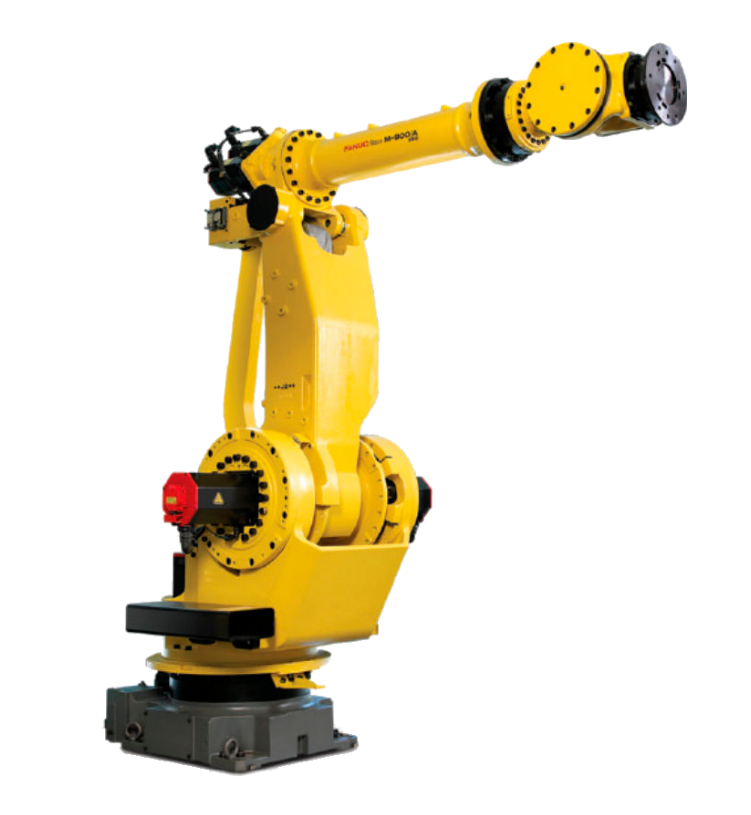
\includegraphics[width=\textwidth, height=\textwidth]{images/robot_industrial.png}
    \caption{Robot industrial}
    \label{fig:f1}
  \end{subfigure}
    \begin{subfigure}[b]{0.25\textwidth}
    \includegraphics[width=\textwidth, height=\textwidth]{images/robot_movil.png}
    \caption{Robot móvil}
    \label{fig:f2}
  	\end{subfigure}
  	\begin{subfigure}[b]{0.25\textwidth}
    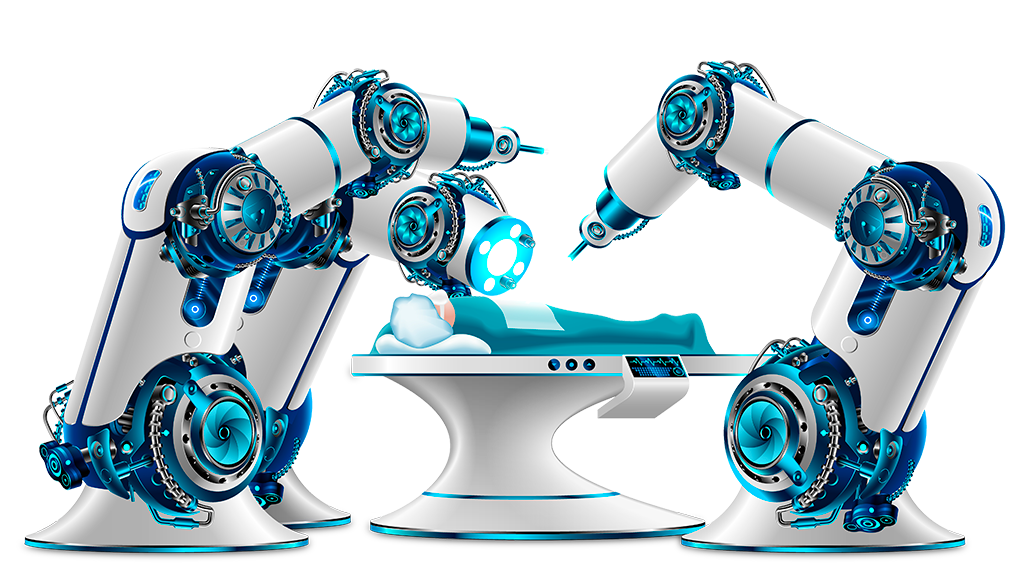
\includegraphics[width=1.3\textwidth, height=\textwidth]{images/robot_medico.png}
    \caption{Robot médico}
    \label{fig:f3}
  	\end{subfigure}
  	\begin{subfigure}[b]{0.25\textwidth}
    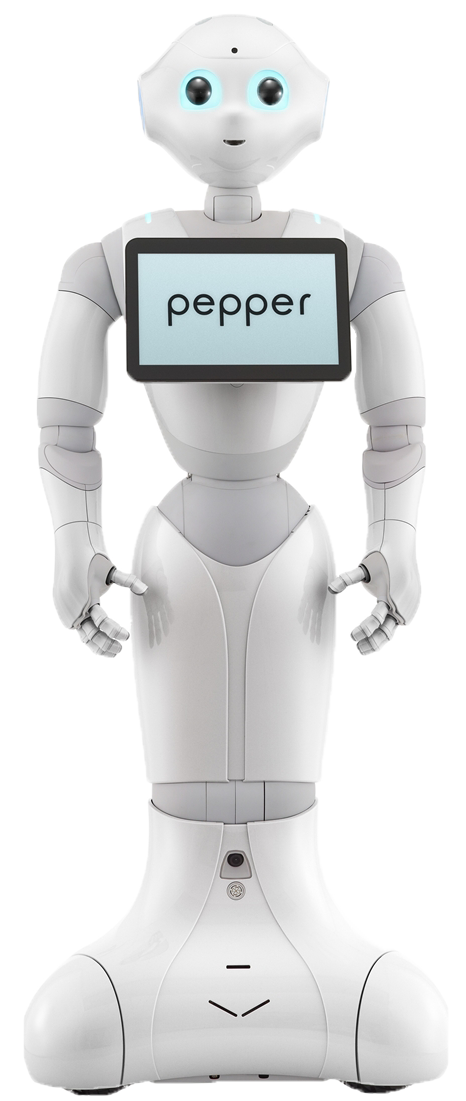
\includegraphics[width=0.7\textwidth, height=\textwidth]{images/robot_androide.png}
    \caption{Robot androide}
    \label{fig:f3}
  	\end{subfigure}
  	\caption{Tipos de robots en función de su utilidad.}
\end{figure}
	\end{itemize}


	\item En función de su operación:
	\begin{itemize}
		\item Robots teleoperados. Aquellos robots que realizan acciones que son controladas de manera remota por una persona. Este tipo de robots se utilizan principalmente en tareas que puedan suponer un riesgo de salud para las personas, pero que al mismo tiempo requieran un tratamiento humano para su elaboración (por ejemplo robots para desactivación de bombas controlados a distancia por una persona).
		
		\item Robots autónomos. Por el contrario, este tipo de robots son capaces de realizar taeras de manera independiente ya que son máquinas mucho más complejas y son dotadas con cierta inteligencia. Este tipo de robots son utilizados en algunos escenarios en los que el robot es capaz de analizar el entorno que le rodea para generar una respuesta por sí mismo. Este tipo de robots es el que utilizaremos para desarrollar este proyecto.
	\end{itemize}
\end{enumerate}

A día de hoy la robótica está presente en casi cualquier ámbito de nuestra vida; desde pequeños robots en el entorno doméstico (como aspiradoras inteligentes o electrodomésticos conectados a Internet) hasta robots que nos facilitan las tareas en nuestro puesto de trabajo (robots médicos, industriales,etc). El campo de la robótica siempre está en continua investigación y desarrollo, ya que el objetivo final de la robótica es mejorar la vida de las personas. Además la tendencia de crear un mundo conectado abre las puertas a la robótica y a robots personalizados que trabajen junto a las personas, creando nuevos puestos de trabajo y mejorando la calidad de los puestos de trabajo existentes. Una vez puesto en valor la importancia de la  robótica en la actualidad, en este trabajo de fin de grado se ha desarrollado una de las posibles aplicaciones de la robótica a un entorno real, dotanto a un robot móvil de la intenligencia necesaria para poder circular en un entorno simulado e ir detectando y analizando su entorno para actuar en consecuencia.


\section{Deep Learning en Visión Artifical}

El \textit{Deep Learning} (aprendizaje profundo) es una rama de la ingeniería que permite a un ordenador crear conceptos y lógicas complejas a partir de otras más simples, todo ello mediante un aprendizaje automático. Es un conjunto de algoritmos que permiten crear un conocimiento en una máquina mediante un entrenamiento, e intentan modelar abstraciones de alto nivel (por ejemplo percepciones humanas tales como identificar distintos objetos en una imagen) utilizando arquitecturas compuestas de transformaciones no lineales múltiples. Una de las grandes ventajas del Deep Learning es que, a medida que aumenta la cantidad de datos y de ejemplos utilizados, mejora la precisión del algoritmo.
\\

En un contexto más amplio, el \textit{Deep Learning} es uno de los subconjuntos de la Inteligencia Artificial, que es la ciencia que estudia la intenligencia llevada a cabo por las máquinas. En términos generales, dentro de la Inteligencia Artificial podemos encontrar el Aprendizaje Máquina (\textit{Machine Learning}, definido como la capacidad de las máquinas para aprender, construyendo modelos o patrones a partir de datos no procesados), el Aprendizaje de la Representacion (\textit{Representation Learning}, que emplea el Aprendizaje Máquina para descubrir automáticamente representaciones o clasificaciones de datos sin procesar) y finalmente el Aprendizaje Profundo (\textit{Deep Learning}). El diagrama de Venn (figura 1.2) muestra los subconjuntos de la Inteligencia Artificial.
\\

\newpage
Por otra parte la Visión Artificial (\textit{Computer Vision} visión por computadora) es la rama de la ciencia que recopila todos los métodos para adquirir, procesar, analizar y comprender las imágenes del mundo real para que puedan ser procesadas por un ordenador. En concreto, en este proyecto combinaremos la visión artificial (obtención de imágenes de un robot de un entorno real simulado) con \textit{Deep Learning} (procesamiento e interpretación de esas imágenes) para dotar de la inteligencia necesaria a un robot y que sea capaz de actuar en función de las condiciones de su entorno. 

\begin{figure}[h]
	\centering
	 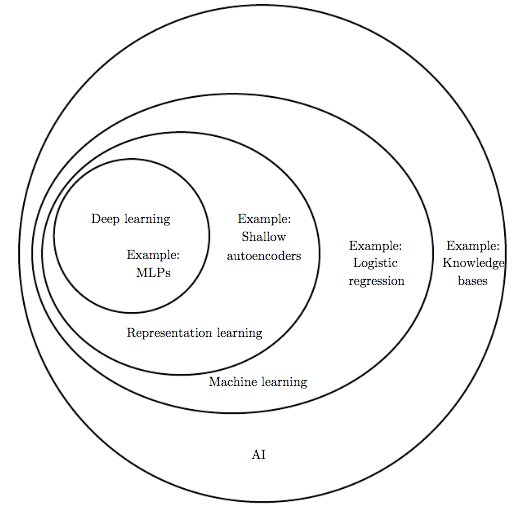
\includegraphics[scale=0.6]{images/diagrama-venn.jpg}
	 \caption{Diagrama de Venn}
\end{figure}

\newpage
\section{Redes Neuronales Convolucionales (CNNs)}

Existen distintas técnicas para llevar a la práctica el \textit{Deep Learning}. Una de ellas son las Redes Neuronales Convolucionales (CNN). Las redes neuronales son modelos de aprendizaje automático que intentan emular las neuronas de los sistemas nerviosos biológicos. Al igual que un cerebro humano, las redes neuronales pretenden establecer conclusiones de los datos que obtienen. En concretro, las Redes Neuronales Convolucionales utilizan filtros convolucionales (múltiples filtros o capas por los que va pasando la información) para realizar esta función.
\\

La arquitectura de las Redes Neuronales Convolucionales se basa en utilizar distintos niveles o capas, en los que despúes de cada uno de ellos se añade una función para realiar un mapeo causal no-lineal. Es decir, cada capa está formada por dos subcapas: una capa convolucional (que realiza una operación de convolución), y una capa de submuestreo (\textit{pooling}, que genera características a partir de cálculos estadísticos del resultado de la convolución). Todas estas capas están conectadas de  tal forma que a la salida de todas ellas se puedan obtener conclusiones a partir de los resultados obtenidos. Cuantas más capas posea una red neuronal, más probabilidad hay de que los resultados obtenidos sean acertados. En la figura 1.3 podemos encontrar un ejemplo de una red neuronal convolucional que clasifica un número manuscrito al número digital que corresponde. 

\begin{figure}[h]
	\centering
	 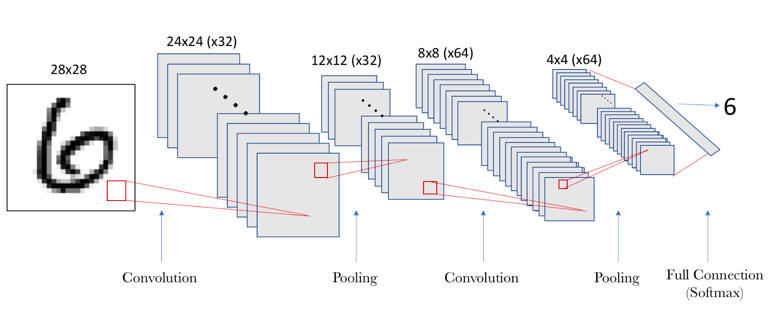
\includegraphics[scale=0.45]{images/ejemplo_cnn.png}
	 \caption{Ejemplo de la arquitectura de una Red Neuronal Convolucional}
\end{figure}

Este trabajo se centra en la detección de objetos a través de imágenes, por lo que las Redes Neuronales Convolucionales son de gran utilidad ya que con ellas se puede procesar la imagen por secciones e identificar los objetos de manera más eficiente. Aplicando una red neuronal convolcional a nuestras imágenes podremos identificar el tamaño, la posición y el tipo de objeto que aparece en una imagen (siempre y cuando la clasificación del objeto identificado se encuentre dentro de las clases determinadas de la red neuronal). Para dicha implementación, existen diversas plataformas tales como Keras, TensorFlow, Caffe, etc. En nuestro caso utilizaremos TensorFLow, y en concreto TensorFlowjs que es la librería para desarollarlo en JavaScript. El motivo de esta elección es que utilizaremos nuestra red en un entorno web, por lo que el hecho de que exista dicha librería en lenguaje JavaScript nos facilitará la incorporación de la red a nuestro entorno. Además TensorFlow dispone de numerosos modelos pre-entrenados que podremos usar sin la necesidad de entrenar previamente un modelo y etiquetar infinidad de imágenes.

\section{Robótica en educación}

En los últimos años ha aumentado de manera exponencial la enseñanza de la róbitca en edades tempranas. Esto se debe a que apreder robótica puede ofrecernos una formación en diversos campos de forma simultánea; física, electrónica, informática...Además el uso de aplicaciones de robótica refuerza la creatividad (a través del diseño de ideas y su desarrollo), el pensanmiento crítico (pensamientos lógicos) y prepara a los niños para un futuro llego de robótica. Es por ello que en estos últimos años se han desarrollado numerosas plataformas orientadas a este fin. Entre ellas podemos encontrar OpenRoberta, iRobot y Kibotics/Websim (que es la que usaremos para este proyecto).

\subsection{OpenRoberta}

Es una plataforma orientada a la programación por bloques en la que se pueden programar robots y otros sistemas hardware programabes como Arduino, BBC micro y Calliope mini. El objetivo de OpenRoberta es simplificar los conceptos de programación para poder introducir la programación en los colegios. Ofrece un entorno de programación basado en la nube (desarrollado en código abierto) que permite su uso en cualquier navegador, sin necesidad de instalación. Dispone de varios robots y sistemas (mBot,Arduino,etc) con múltiples motores y sensores que pueden ser configurados a través de bloques. Ofrece múltiples idiomas y no es necesario registrarse para utilizarlo.

\begin{figure}[h]
	\centering
	 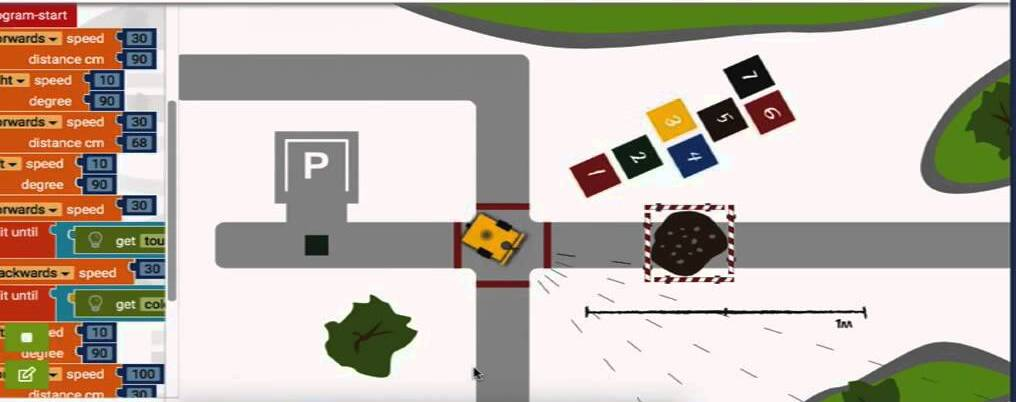
\includegraphics[scale=0.4]{images/openRoberta.jpg}
	 \caption{Interfaz de OpenRoberta}
\end{figure}


\subsection{iRobot}

iRobot es una empresa estadounidense que se dedica al diseño y fabricación de robots, principalmente orientados al uso en empresas, hogares e instituciones. Es conocida por el robot \textit{Roomba}, un aspirador doméstico inteligente. Esta empresa ha creado un robot móvil llamado Create2 destinado a que los estudiantes y desarrolladores puedan programar los movimientos y el comportamiento del mismo. Está destinado a estudiantes de secundaria y universidad, para que puedan empezar a adquirir experiencia en programación y comprender los conceptos de robótica.

\begin{figure}[h]
	\centering
	 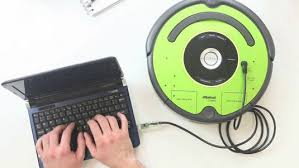
\includegraphics[scale=0.8]{images/irobot.jpeg}
	 \caption{Robot Create2 de iRobot}
\end{figure}

\subsection{Kibotics/Websim}

Es una plataforma desarrollada por la Asociación de robótica e inteligencia artificial JdeRobot, destinada a la docencia en robótica y programación (\textit{STEM: Science, Technology, Engineering, Mathematics}). El objetivo de Kibotics es iniciar a niñ@s y adolescentes en robótica y programación de robots. No necesita instalación ya que se despliega en el navegador. Utiliza lenguajes Python y Scratch. Es especialmente interesante porque ofrece una gran variedad de robots programables tanto reales como simulados (PiBot, drones, Fórmula 1), y permite el desarrollo de prácticas con visión artificial (robots con cámara). Esta es la plataforma que se va a utilizar para desarrollar este TFG.

\begin{figure}[h]
	\centering
	 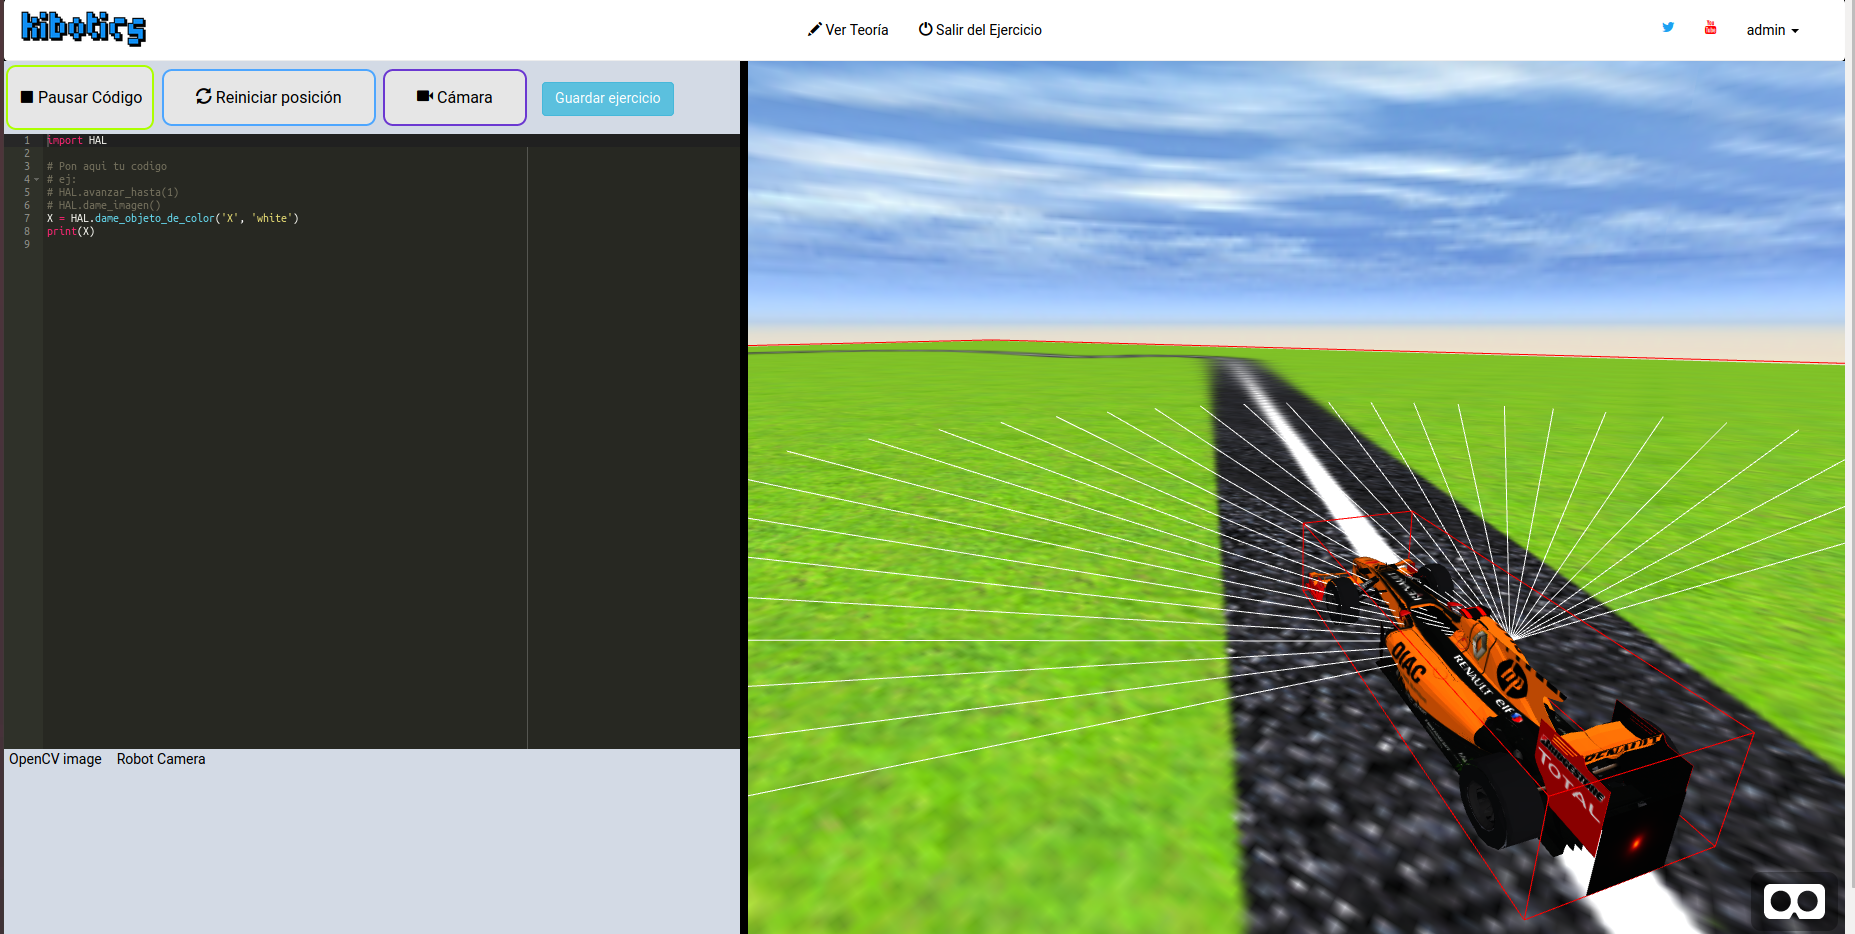
\includegraphics[scale=0.15]{images/kibotics.png}
	 \caption{Interfaz de Kibotics}
\end{figure}



\chapter{Objetivos}

\section{Objetivos}
\section{Metodología}
\section{Requerimientos}

\chapter{Infraestructura}
\section{Websim}
\subsection{RobotAPI, Worker and Miniproxy}
\section{Biblioteca OpenCVjs}
\section{Biblioteca TensorFlowjs}
\section{Blender}

\chapter{Robot Autónomo en Ciudad Simulada}
\section{PiBot}
\section{Ciudad Simulada}
\subsection{Alfombra Infantil}
\subsection{Señales de tráfico}
\subsection{Semáforo animado}
\subsection{Peatones animados}
\section{Sigue-Carretera Básico}
\subsection{Percepción}
\subsection{Actuación}
\section{Sigue-Carretera Avanzado}
\subsection{Modelos de Redes Neuronales}
\subsubsection{MNIST}
\subsubsection{COCO-SSD}
\subsection{Percepción}
\subsection{Actuación}

\chapter{Conclusiones}
\subsection{Conclusiones}
\subsection{Líneas futuras}

\chapter{Bibliografía}

\end{document}
